\section{Semaine 3 - 19 fev}

\subsection{Lundi}

Normalement on allait obtenir l'optimization pour les antennes, mais on n'arrive même pas à
réproduire les résultats de Matthias Pacé. Demain on va continuer.

\subsection{Mardi}

On n'arrive pas a trouver les mêmes résultats que Matthias. Parce qu'on n'arrive pas avec le bowtie, on a
decidé d'essayer d'abord avec l'antenne dipolaire. Je ne suis pas arrivé à le faire. C'est Mathieu qui a 
trouvé la solution, montrée sur la Figure \ref{fig:first_dipole}. En fait il fallait construire le port à 
travers le mode \textit{pick edge}. Je ne suis pas sûr de pourquoi ca change tellement.
J'ai dans mes notes une formule pour calculer l'impendance du port, et je suis arrivé a obtenir l'impendance
correcte pour l'antenne de bowtie, mais je ne comprends pas la formule.

\begin{wrapfigure}{R}{0.4\textwidth}
    \centering
    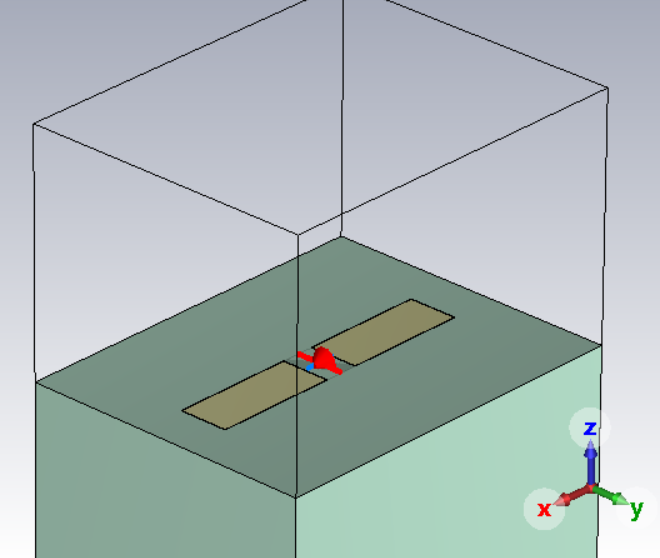
\includegraphics[width=0.35\textwidth]{texfigures/first_dipole.png}
    \caption{\label{fig:first_dipole} Une antenne dipolaire en or sur un subtrat de saphire 
    (Alumina au $96\%$ sans pertes). Les dimensions son $57\mu $m pour la longueur totale De
    l'antenne, $7\mu $m pour le gap, $10\mu $m pour la base de l'antenne, $0.1\mu $m pour l'épaisseur.}
\end{wrapfigure}

Victor a codé pendant toute la journée. On a aussi commencé à travailler avec GitHub. On a aussi assisté
à un séminaire sur des modèles théoriques pour la création de nouveaux pigments. C'était intéressant.